\documentclass[14pt]{beamer}
\usepackage[T1]{fontenc}
\usepackage[utf8]{inputenc}
\usepackage[slovene]{babel}
\usepackage{pgfpages} % privat zapiski
\usepackage{amsmath} % pravilen izpis v "math mode"
\usepackage{hyperref}
\usepackage{pgfplots}
\usepackage{tikz}
%\documentclass{standalone}
%\usepackage{pgfplotstable,filecontents}

\pgfplotsset{compat=1.8}
\hypersetup{hidelinks}
%\usetheme{Bergen}
\usecolortheme{seahorse}

\usepackage{graphicx}% http://ctan.org/pkg/graphicx
\usepackage{booktabs}% http://ctan.org/pkg/booktabs

\usepackage{palatino}
\usefonttheme{serif}

\setbeamertemplate{navigation symbols}{} % izklop navigacije
\setbeamertemplate{footline}[frame number]{} % oštevilčenje
\setbeamertemplate{note page}{\pagecolor{yellow!5}\insertnote}
\setbeamertemplate{itemize items}[circle]



\begin{document}
    \title[Diplomski seminar]{Iterativne numerične metode v posplošenih linearnih modelih}
    \author[Mitek]{Mitja Mandić \\ \small Mentor: izred. prof. dr. Jaka Smrekar}
    \date{20. november 2020} 

\begin{frame}
    \titlepage
\end{frame}

\begin{frame} \frametitle{Posplošeni linearni modeli}
    \begin{itemize}
    
        \item Slučajni del, sistematični del, povezovalna funkcija
        \pause
        \item Linearna regresija: 
            $$ Y = x ^ T\beta $$
        \item Problem - ni najboljša. Rešitev? Transformacija Y
    \end{itemize}
\end{frame}

\begin{frame} \frametitle{Logistični model}
    \begin{itemize}
    \item Za kategorične podatke $\rightarrow$ binomska porazdelitev
    \pause
    \item $ \mathrm{logit}(p_{i}) = \mathrm{log} (\frac{p_{i}}{1 - p_{i}}) = x ^ T\beta $ %\rightarrow p_{i} = \frac{ e^{x^T\beta}}{1 + e^{x^T\beta}} $
    %\item Sedaj je treba izračunati $\beta$ $\rightarrow$ Numerične metode

    \end{itemize}
\end{frame}

\begin{frame}


$$p = \frac{e^{x^T\beta}}{1+e^{x^T\beta}}$$
\begin{figure}   % treba še naštudirat da bo graf prou
\begin{center}
    \begin{tikzpicture}
        
        \begin{axis}%
        [
            grid=major,     
            xmin=-10,
            xmax=10,
            axis x line=bottom,
            ytick={0,.5,1},
            ymax=1,
            axis y line=middle,
        ]
            \addplot%
            [
                blue,%
                mark=none,
                samples=100,
                domain=-6:6,
            ]
            (x,{1/(1+exp(-x))});
        \end{axis}
    \end{tikzpicture}

\end{center}
\end{figure}
\end{frame}


\begin{frame}\frametitle{Numerične metode}
    \begin{itemize}
        \item Za ocenjevanje parametrov $\beta$ običajno rešujemo sistem enačb največjega verjetja
        \pause
        %\item v splošnem ni eksplicitno rešljiv
        \item Newtonova metoda še vedno zelo aktualna:
        $$ x_{i+1} = x_{i} - \frac{f'(x_{i})}{f''(x_{i})} $$
        %\pause
        
        \item Izboljšava: Fisher-scoring  
    \end{itemize}
\end{frame}

\begin{frame}{Fisher scoring}

    $$ \beta_{i+1} = \beta_{i} + \frac{\dot{l}(\beta_{i})}{E(\ddot{l}(\beta_{i}))} $$
    
    \begin{itemize}
        \item za logistično regresijo sovpadata z Newtonovo metodo
        \item Informacijska matrika je pozitivno definitna $\rightarrow$ imamo naraščajoč algoritem
    \end{itemize}

\end{frame}

\begin{frame}{Fisher scoring za logistični model}
    \begin{gather*}
        \hat{\beta}_{i+1} = \hat{\beta}_{i} + (X^T  v(\hat{\beta}_{i}) X) ^{-1}  X^T (y - \mu(\hat{\beta}_{i})) \\
         = \hat{\beta}_{i} + \text{(inverz info)(score)}
    \end{gather*}
    \pause
    Računanje inverza je lahko problematično. To rešimo takole:
    \begin{gather*}
        h = \hat{\beta}_{i+1} - \hat{\beta}_{i} \\
        X^T  v(\hat{\beta}_{i}) X = h * X^T (y - \mu(\hat{\beta}_{i}))
    \end{gather*}
\end{frame}

\begin{frame}{Challenger podatki}
    \centering
    $p = \frac{e^{15.04290 - 0.23216x}}{1+e^{15.04290 - 0.23216x}}$
\begin{figure}
    \centering
    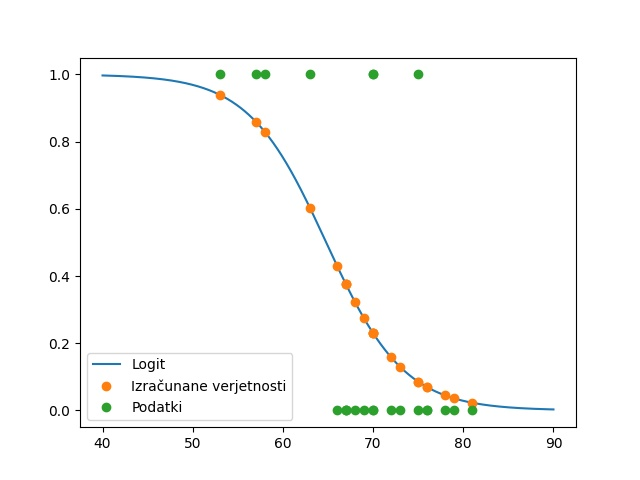
\includegraphics[scale=0.6]{logit_challenger.jpeg}
\end{figure}

\end{frame}

\begin{frame}{Kaj še bom naredil}
    \begin{itemize}
        \item Analiziral časovno zahtevnost že postavljenega algoritma
        \item Izvedel podobno še za kak drugačen model
        \item Teorijo razvil še za splošen posplošen linearen model
    \end{itemize}
\end{frame}
\end{document}